\documentclass[draftmode,draftwater]{memarticle}
%\documentclass[screen,nopanel]{memarticle}
%\documentclass{memarticle}
\usepackage{paralist}
\usepackage[T1]{fontenc}
\usepackage{palatino%
           , pxfonts%
           , mathpazo%
           }
\maxtocdepth{chapter}

%------------------------------------------------------------
% Document title control. Change these as appropriate for your
% document.
%------------------------------------------------------------
\newcommand{\doctitle}{A Proposal for \\ a DES Parameter Estimation System}
\newcommand{\brieftitle}{CosmoSIS}
\newcommand{\authors}{\href{mailto:jbk@fnal.gov,paterno@fnal.gov}%
                     {Jim Kowalkowski and Marc Paterno \\ \textit{Computing Division} \\ \textit{SSI Group}}}
\newcommand{\docversion}{12}

%------------------------------------------------------------
% Define new commands here
%------------------------------------------------------------
%\newcommand{\despes}{\name{despes}\xspace}
\newcommand{\facs}{\name{FACS}\xspace}
\newcommand{\cosmosis}{\name{CosmoSIS}\xspace}


%------------------------------------------------------------
% Document starts here
%------------------------------------------------------------
\listfiles
\begin{document}
	
\topmatter	% include this to typeset the title, authors, and toc.

%------------------------------------------------------------
\chapter{Introduction\label{ch:introduction}}

\section{Purpose\label{sec:purpose}}

This document describes the features and properties of a proposed
software system, containing several elements:
\begin{inparaenum}[(a)]
\item a framework for the construction of runtime-configurable,
parallel-capable, Markov Chain Monte Carlo (MCMC)-based parameter estimation programs, which we
call \cosmosis (Cosmological Survey Inference System). This framework is initially targeted for the Dark Energy
Survey (DES)\cite{des} project,
\item software libraries to support assembly of applications using this
  framework, and
\item a development environment to assist with collaborative development
 of such libraries, including repository use, software packaging, and
 deployment of packaged software.
\end{inparaenum}

\cosmosis will support parallel execution through a multi-process (as
opposed to multi-threaded) model, while still allowing (but not
requiring) individual bodies of code to be internally
multi-threaded. This will allow users of the framework to take
advantage of modern multi-core platforms, without requiring that
physicists---who program the modules that run within
the framework---deal with the intricacies of multi-threaded
programming.

The major purpose of this document is to provide a clear description
of the project and to obtain agreement on its constraints,
essential requirements, and current state.  The later sections will
propose a high-level design of the system that will meet the overall goals.

%  It is the result of two days' discussion
% between the authors, Scott Dodelson (Fermilab), Elizabeth Buckley-Geer
% (Fermilab), and Joe Zuntz (Oxford), which took place August~1--2,
% 2012.

This document is intended for all the stakeholders in the project, as
well as for potential users of the software described.

% Describe what it is this report is going to convey or what this paper
% is about. Define the system that is being described and interesting
% qualities such as whether or not it is a utility to be shared by many.
% Include what this report should not include.

\section{Scope\label{sec:scope}}

This document describes the primary aspects of the proposed software
products and practices for using them. These include:

\begin{itemize}

\item A modular software \emph{framework} (\cosmosis) for building \emph{MCMC-based
   parameter estimation programs} for dark energy science. This
  framework will be suitable for use by physicists participating in the
  Dark Energy Survey, and eventually by others as well. The framework
  will be developed under the DOE Computational HEP \facs proposal.
  It will
  support the development, configuration and use of
  user-supplied MCMC samplers, likelihood calculators, and physics
  calculators.

\item A collection of application programming interfaces (APIs) that
  define how the modular elements of the framework program are
  configured, how they obtain their input data, how they interact, and
  how new modular components can be added to the system.

  Module types include \emph{samplers}, \emph{physics calculators}, and
  \emph{likelihood calculators}. The module API will support
  multi-threaded operation.

 % Per email from Joe Zuntz, support of legacy stand-alone calculators
 % is not needed.
 % Standard physics calculator modules will be
 %  provided to support legacy stand-alone programs, using multi-process
 %  parallelism. \ifixme{Is there also a need for a standard likelihood
 %    module, to invoke legacy stand-alone likelihood calculation
 %    programs?}

  APIs for physics modules, likelihood modules, and samplers will be provided in
  \cpp{}11, C99\footnote{C99 is chosen, rather than C11, for better
    compatibility with \cpp{}11; the C99 standard is part of the
    \cpp{}11 standard.}, Fortran 90, and Python 2.7.

\item A system for organizing and maintaining source control over the
  software produced by DES for this purpose. The \cosmosis framework code
  itself will reside in one repository. For each package of related
  modules, a separate source code repository will be created.

\item A system for building and testing of the source code over which we
  have control.\footnote{Third-party libraries will be built using their
    own build systems, and delivered through our product delivery
    system.} Because Python has a native build system, and a widely
  popular testing system, the system used for building and testing
  Python may be different from the system used for building and testing
  code in the compiled languages.

\item A system for distribution of software used by \cosmosis, including
  software written by DES and software written by others and used by
  \cosmosis (\eg, the GNU compiler suite, the Python interpreter, and
  \name{NumPy}~\cite{numpy}).

\item A system for organizing the data files used as input for the
  parameter estimation process.

\item A system for structuring the output files of the parameter
  estimation process. This structured output includes a scheme for
  automatic tracking of the provenance of the generated samples.

\end{itemize}

% Indicate the boundaries of this subsystem and also for this
% report. This section includes information about what is covered in the
% report and examples of what is not.

\section{Rationale\label{sec:rationale}}

The dark energy science analysis done by DES will involve a large enough
group of physicists
that independent and uncoordinated development will be inefficient. In order to
avoid duplicated effort, and in order to allow members of the
DES Dark Energy Science Center collaborate more easily, we propose the
development of an organized environment for cosmological parameter
estimation.
\begin{fixme}
  Is ``the DES DESC'' the right group to name here, or is that too
  specific, or too general?
\end{fixme}

At the highest level, the goal of this effort is to create a
collaborative environment in which dark energy science
analysis\footnote{This effort will begin by focusing on Markov Chain
  Monte Carlo likelihood sampling analyses.} can
be performed. The environment should be easy to deploy to a new computer,
as long as the computer is running one of the experiment-supported
operating systems. It should be easy for a physicist to introduce new
physics algorithms into the parameter estimation process, or to
replace an existing algorithm by a different implementation. It should
also be easy to ensure that large jobs can take advantage of
parallel-processing opportunities on multi-core machines, without
requiring significant parallel-programming experience on the part of
the physicist-programmers.

\section{Terminology\label{sec:terminology}}

In this section, we introduce some technical terminology used
elsewhere in the document.

\begin{description}

\item[Application programming interface] An \emph{application
    programming interface} (API) is a set of data structure and function
  signature definitions, along with the specification of the behavior of
  the functions.

\item[Configuration file] A \emph{configuration file} is file (usually
  a text file) that provides parameters necessary for the execution of
  a program. These are sometimes called \emph{initialization files}.

\item[Distribution system] A (binary) \emph{distribution system} is a
  means for the delivery of \emph{libraries}, \emph{programs},
  \emph{modules} and \emph{headers} (and possibly other associated
  artifacts, such as configuration files), to users. Contrast with a
  \emph{repository}.

\item[Dynamic library] A \emph{dynamic library} is a \emph{library} that
  is linked with at run-time, as opposed to (static) linking time. The
  use of dynamic libraries allows some functions of a program to be
  replaced without rebuilding the entire program.

\item[External product] An \emph{external product} is a body of software
  used by another software product, but which is not built as part of
  that other product.

\item[Framework] A \emph{framework} is a software system used to
  create a program for a specific purpose. A framework typically
  provides a means to allow the integration of user-written code into
  the program, often as \emph{dynamic libraries}.
  A framework typically provides the \code{main} function
  for the program. Contrast with a \emph{toolkit}.

\item[Header] A \emph{header} is a source code file, used in C and
  \cpp, to introduce prototypes of functions and definition of
  \code{struct}s or \code{class}es. In \cpp, some codes (\eg,
  template-based ``libraries'') consist entirely of headers.

\item[Library] A \emph{library} is a body of compiled code,
  encompassing a collection of functions intended for use in building
  other libraries or programs.

\item[Likelihood calculator] A \emph{likelihood calculator} is a module
  that has the purpose of calculating, based on the values if its
  \emph{input} physics parameters, a set of \emph{output} physics parameters.
  See also \emph{physics calculator}.

\item[Module] A \emph{module} is a body of code which presents a set
  of classes, or functions, or both. Modules can consist of pure
  Python (in which case no platform dependence in the build will
  appear), or as compiled extension modules (in which case the built
  module is platform-dependent), or as a mixture of the two.

\item[Physics calculator]
See also \emph{likelihood calculator}.

\item[Platform] A \emph{platform} is a particular combination of
  computing hardware and operating system version. It includes many
  ``standard'' tools, \eg, \code{make}.

\item[Program] A \emph{program} is a utility to be
  invoked from the command line, or as part of a batch job. It may be
  compiled (as are Fortran and C programs) or interpreted (as are
  Python programs). Contrast with a \emph{library}.

\item[Repository] A (source code) \emph{repository} is a system used
  for the version control of source code. Contrast with a
  \emph{distribution system}.

\item[Toolkit] A \emph{toolkit} is a software system, typically a
  library, module, or set of libraries or modules or both, that
  provides utilities (functions, \code{struct}s, and \code{class}es)
  to be used by user-written code. Contrast with a \emph{framework}.

\end{description}

\chapter{Essential features}

Here we describe the various aspects of the software
system, the essential functions that it must support, and the
constraints to which is must adhere. In earlier proposals and
discussions, we have referred to this this project as a framework. It
is, however, more appropriately called a system since it also encompasses
developing and running the applications that use the libraries and
software modules. This section contains rules and mandates that we
must follow (constraints) and essential functions that the system must
carry out (functional requirements).

\section{Roles that people play}

Here we focus on who makes use of this system and what sort of
activities they do. We have identified four main roles related to the
\cosmosis software. The activities performed by scientists acting in
these roles are the primary focuses of this project. It is important to
note that the same person may, at different times, more from one role to
another. The main roles are:
\begin{description}

\item[Scientist user]: \emph{Scientist users} (henceforth just
  \emph{users}) make use of programs and libraries that are already
  installed. They configure programs, select input data sets, and run
  jobs. When doing analysis, scientists are often acting in the
  \emph{user} role. This can be true even when one is using code one has
  previously developed.

\item[Scientist developer]: \emph{Scientist developers} (henceforth just
  \emph{developers} write, build, and test code, and usually make that
  code available for others to use. When acting in the developer role
  for one body of code, one is often also acting in the user role for
  other code; \eg a developer making use of a given sampler is most
  often not modifying the source code of the sampler, and would thus be
  acting in the user role in respect to the sampler.

\item[Build manager]: \emph{Build managers} create ``offical''
  distributions of software, and make those distributions available for
  others to obtain. They may also create site-specific builds of
  software, when necessary.

\item[Install manager]: \emph{Installation managers} install
  ``official'' distributions of software on computing resources for
  which they are responsible. This role might be fulfilled by an
  individual supporting a group at a national laboratory or at a
  university, or by an individual installing software on his own laptop.

\end{description}

\section{Work sequence examples}

There are several development and runtime scenarios (or work
sequences) that will help focus and describe the needs that this new system will
address.

\subsection{Configuring and running existing software}
\subsection{Modifying an existing physics module}
\subsection{Creating a new physics module}
\subsection{Creating an official release}
\subsection{Installing a new release}

\section{Software categories}

Software added to the system falls into several categories: platform,
external, core, contributions. This section defined each of these
categories and describes their constraints and essential requirements.

These categories are arranged in a hierarchy of dependencies: platform
software can depend only on other platform software; external software
can depend upon other external software and on platform software; core
software can depend on other core software, and on external and platform
software; contribution software can depend on other contribution
software, and on anything in any of the other categories.

\subsection{Platform}

Platform software elements are those elements which are not delivered
through the software product distribution system, but are required as
part of the software inherent on a given platform. Some examples would
be the \texttt{bash} shell, and the system's standard C library
(\texttt{libc.so} on Linux systems, \texttt{libSystem.dylib} on Darwin
systems).

\subsection{External}

External software elements are those elements distributed through the
software product distribution system, but which are not created from
software controlled by the project (\eg the Python interpreter and the
GNU Scientific Library). Typically they have their own system for
building the software.

Such software elements will be built using their own build system, and
packaged into the form used by the product distribution system.

\subsection{Core}

Core software elements are those elements that are part of the project,
and are used by scientist-developer written code, but which do not
(often) need modification by scientist developers.

\subsection{Contribution}

Contribution software elements are those elements that are part of a
collaboration's code. They are the software elements with the ``physics
knowledge'' of the system, and are primarily developed by scientists.

\section{Run-time environment}

The subsystems that permit one to use the developed software and other
externally developed applications and tools to solve problems are
contained in this section. This section defines each of these
subsystems and describes their constraints and essential requirements.

\subsection{Runtime configuration}

\subsection{Data repositories}

\subsection{Configuration repositories}

\subsection{Package repositories}

\subsection{Environment settings}

\subsection{Data handling interface}

\subsection{Platform interactions for special facilities} 

\section{Development environment}

The subsystems that permit software development activities and house
software artifacts are contained in this section. This section defines
each of these subsystems and describes their constraints and essential
requirements.


\subsection{Source code repositories}

\subsection{Build, test, package, and local install}


\subsection{Distribution repositories}


\section{Project-wide constraints}

\subsection{Supported platforms}

For all supported platforms, there will be regular releases of the
project's software that are centrally built and made available for
distribution. On a best-effort basis, we will try to maintain code
portability so that interested users can build their own releases on
unsupported systems, but releases for unsupported systems will not be
centrally created and distributed.

The set of supported platforms includes:
\begin{enumerate}
   \item Scientific Linux Fermi 6.x, on x86-64 hardware, in 64-bit mode.
   \item Scientific Linux Fermi 5.x, on x86-64 hardware, in 64-bit mode.
   \item Darwin 10.x (as shipped with Mac OS~X 10.6, ``Snow Leopard''),
     on x86-64 hardware, in 64-bit mode.
   \item Darwin 11.x (as shipped with Mac OS~X 10.7, ``Lion''), on
     x86-64 hardware, in 64-bit mode.
   \item Darwin 12.x (as shipped with OS~X 10.8\footnote{The ``Mac'' has
     apparently been dropped from the operating system name as of
     Mountain Lion.}, ``Mountain Lion''), on
     x86-64 hardware, in 64-bit mode.
   \item Ubuntu 12.x~LTS ``Precise Pengolin'', on x86-64 hardware, in
     64-bit node.
\end{enumerate}

\subsection{Supported shell}

On all supported platforms, the runtime and development environments
will require use of the bash shell, version~3 or newer. This is to avoid
the need to maintain a multiplicity of scripts for these environments,
with the risk that the script might provide subtly different behavior.

\subsection{Supported compilers}

In order to assure compatibility of delivered software products, and to
allow us to upgrade our choice of compilers on our own timescale, the
build system will not make use of the platform-supplied compiler or
Python interpreter. Instead, the compiler suite and the Python
interpreter will be supplied as a UPS product, for each of the supported
platforms.

For all supported compilers, on each platform for which the compiler is
supported, there will be regular releases of the project's software that
are centrally built and made available for distribution.

The set of supported compilers includes:
\begin{enumerate}
  \item The GNU \cpp{}, C and Fortran compilers, from GCC 4.7.3.
  \item Python 2.7.3.
\end{enumerate}
Newer versions of the GNU compilers will be used when they become
available. Newer versions of Python 2.7 will be used when they become
available. Python 3.x will not be supported, because of its
incompatibility with some of the Python modules of interest for the
scientific community.

Non-free compilers will not be officially supported, because they can
not be freely distributed. However, on a best-effort basis, we will try
to keep the build system able to support important commercial compilers,
so that individuals or sites which have licenses to those compiler can
build the software on their own computing resources.

\subsection{Language standards}

Using defined standards for the supported languages, when possible, aids
in the portability of code, making it more certain that code written in
one environment will build and run correctly in other environments.
However, not all language standards are equivalently useful.

\subsubsection{C programming language}

For C we will support the C99 language standard. This language standard
is fully supported by the GNU compiler suite, version 4.7, and is widely
supported by other compilers as well.

\subsubsection{\cpp{} programming language}

For \cpp{} we will support the \cpp{}11 language standard, in the subset
supported by the GNU compiler suite, version 4.7. This is the newest
\cpp{} standard, and while it is not yet completely supported by any
compiler, the (large) fraction of features supported by GCC is
sufficiently valuable to be worth its use.

\subsubsection{Fortran programming language}

For Fortran, we will support Fortran~90 with the additions of TR-15581
(which adds enhanced data type facilities), plus the following list of
features from Fortran~2003:
\begin{enumerate}
\item procedure pointers,
\item IEEE exceptional values,
\item C interoperability features: the \texttt{ISO\_C\_BINDING} module and
  the \texttt{bind} and \texttt{value} attributes.
\end{enumerate}

\subsubsection{Python programming language}

For Python, we will support only the CPython interpreter (not, \eg, the
JVM-based Jython). We will support Python 2.7. On a best-effort bases,
we will try to keep code that will also be compatible with Python 3.x,
to reduce the work that would be necessary if, at some future date, the
community decides to move to using Python 3.

\chapter{Overview\label{ch:overview}}

% \begin{fixme}
%   Things to discuss in this section:
%   \begin{itemize}
% \item concepts
% \item current system architecture
% \item current development methods
% \item current method of running programs
% \item areas we discussion (tools, techniques, components)
% \item what items are most important?
% \item possible changes (differences between what they have and what we propose)
% \end{itemize}
% \end{fixme}

\section{The current situation\label{sec:current_situation}}

The current DES parameter estimation software, residing in the
\texttt{des-pipe} repository, consists of a variety of software
artifacts, written in C99\footnote{The project makefiles typically, but
  perhaps not uniformly, set \texttt{-std=c99}.},
Fortran~90\footnote{Inspection of the source code shows use of features
  removed in Fortran~95, \eg, the \texttt{PAUSE} statement. However, the
  project makefiles do not specify a standard; thus the gfortran default
  of \texttt{-std=gnu} is used, which specifies a superset of the
  Fortran 95 standard that includes all of the extensions supported by
  GNU Fortran, although warnings will be given for obsolete extensions
  not recommended for use in new code. Elsewhere in the code is
use of \texttt{USE ISO\_C\_BINDING}, which is a Fortran~2003 feature
(and a GNU extension in earlier versions of gfortran). The Fortran
language variant used in the code base is not precisely defined.},
 and Python\footnote{The project makefiles indicate a requirement of
   Python 2.6 or Python 2.7.}.
Some of these consist of code written by DES members, others are code
written by others in the astrophysics community, and others are code
written by those outside the community, but all of which have been
imported into the \texttt{des-pipe} source code repository. Some software artifacts are
\emph{programs}, others are (Python) \emph{modules}, while others are
\emph{libraries}. Figure~\ref{fig:astropackages} shows the dependencies
between the software packages currently used by DES parameter estimation
programs.

\subsection{Current external dependencies}

Code in the \texttt{des-pipe} repository depends upon several different
external products. These are not delivered as part of the
\texttt{des-pipe} system; each must be installed by other means. The
required products include:
\begin{enumerate}
  \item A C99 compiler.
  \item A Fortran~90 compiler.
  \item \name{CFITSIO}. The exact version required is unclear.
  \item A Python interpreter, either version 2.6 or version 2.7. Only
    CPython can be used, because of the widespread dependence on
    \name{NumPy}, which does not support alternative Python
    implementations.
  \item \name{NumPy}. The exact version required is unclear, but it must
    be built against the correct Python version. \name{NumPy} has
    optional pieces (\eg, \texttt{numpy.numarray.image}); it is not
    clear which are required.
  \item \name{PyFITS}. The exact version required is unclear, but it
    must be build against the correct Python version.
  \item \name{matplotlib}. The exact version required is unclear, but it
    must be build against the correct Python version. \name{matplotlib}
    depends upon \name{libpng} and \name{freetype}. Since this tool
    supports multiple optional user-interface toolkits, the exact set to
    be supported must be defined.
  \item \name{SciPy}. The exact version required is unclear, but it must
    be built against the correct Python version and using the correct
    \cpp{} compiler. \name{SciPy} involves several other dependencies,
    which we do not elaborate further here: \name{SuiteSparse},
    \name{pcre}, and \name{swig}. \name{SciPy} has optional parts; it is
    not clear which are needed.
  \item \name{emcee}. The exact version required is unclear, but it must
    be built against the correct Python version. \name{emcee} requires
    \name{mpi4py} for full utility, but can work without it; it also
    requires \name{NumPy}. As of version 1.1, \name{emcee} is compatible
    with Python 3. The version current as May~7, 2013 is 1.2.
  \item \name{PyMC}. The exact version required is unclear, but it must
    be built against the correct Python version. It requires
    \name{SciPy}, \name{matplotlib}, and \name{pydot}. It seems that
    \name{PyMC} 2.2 and newer support Python 3\footnote{This is based
      upon commit messages in the PyMC project git repository.}.
\end{enumerate}

\subsection{Current internal dependencies}

The \texttt{des-pipe} software is stored in a single
Mercurial\cite{mercurial} repository, hosted at
BitBucket\cite{bitbucket}. This repository includes some source code
from third parties, imported into the repository.

Figure~\ref{fig:astropackages} shows the dependency graph of the various
named products.

\ifthenelse{\boolean{screen}}{\clearpage}{}
\begin{figure}
  \centering
  \ifthenelse{\boolean{screen}}
{%
  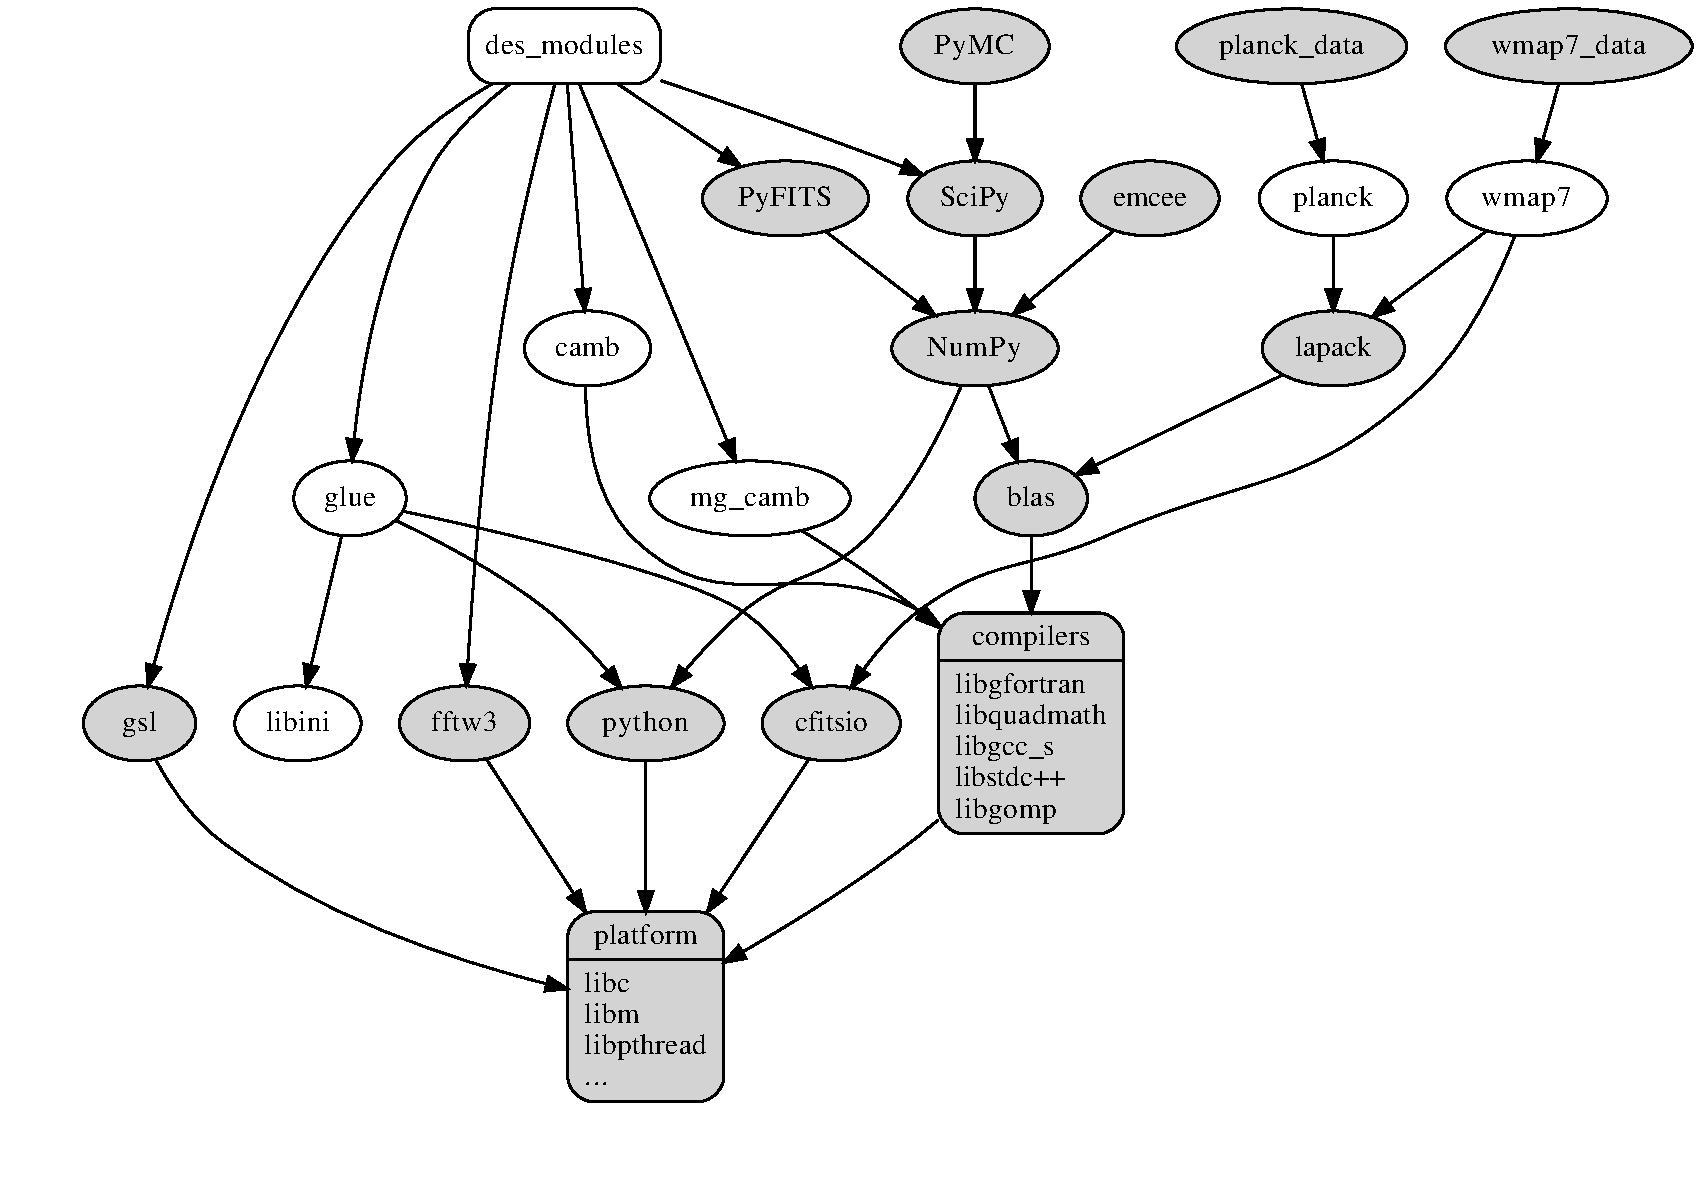
\includegraphics[width=0.95\textheight]{astro_packages}
}{%
  %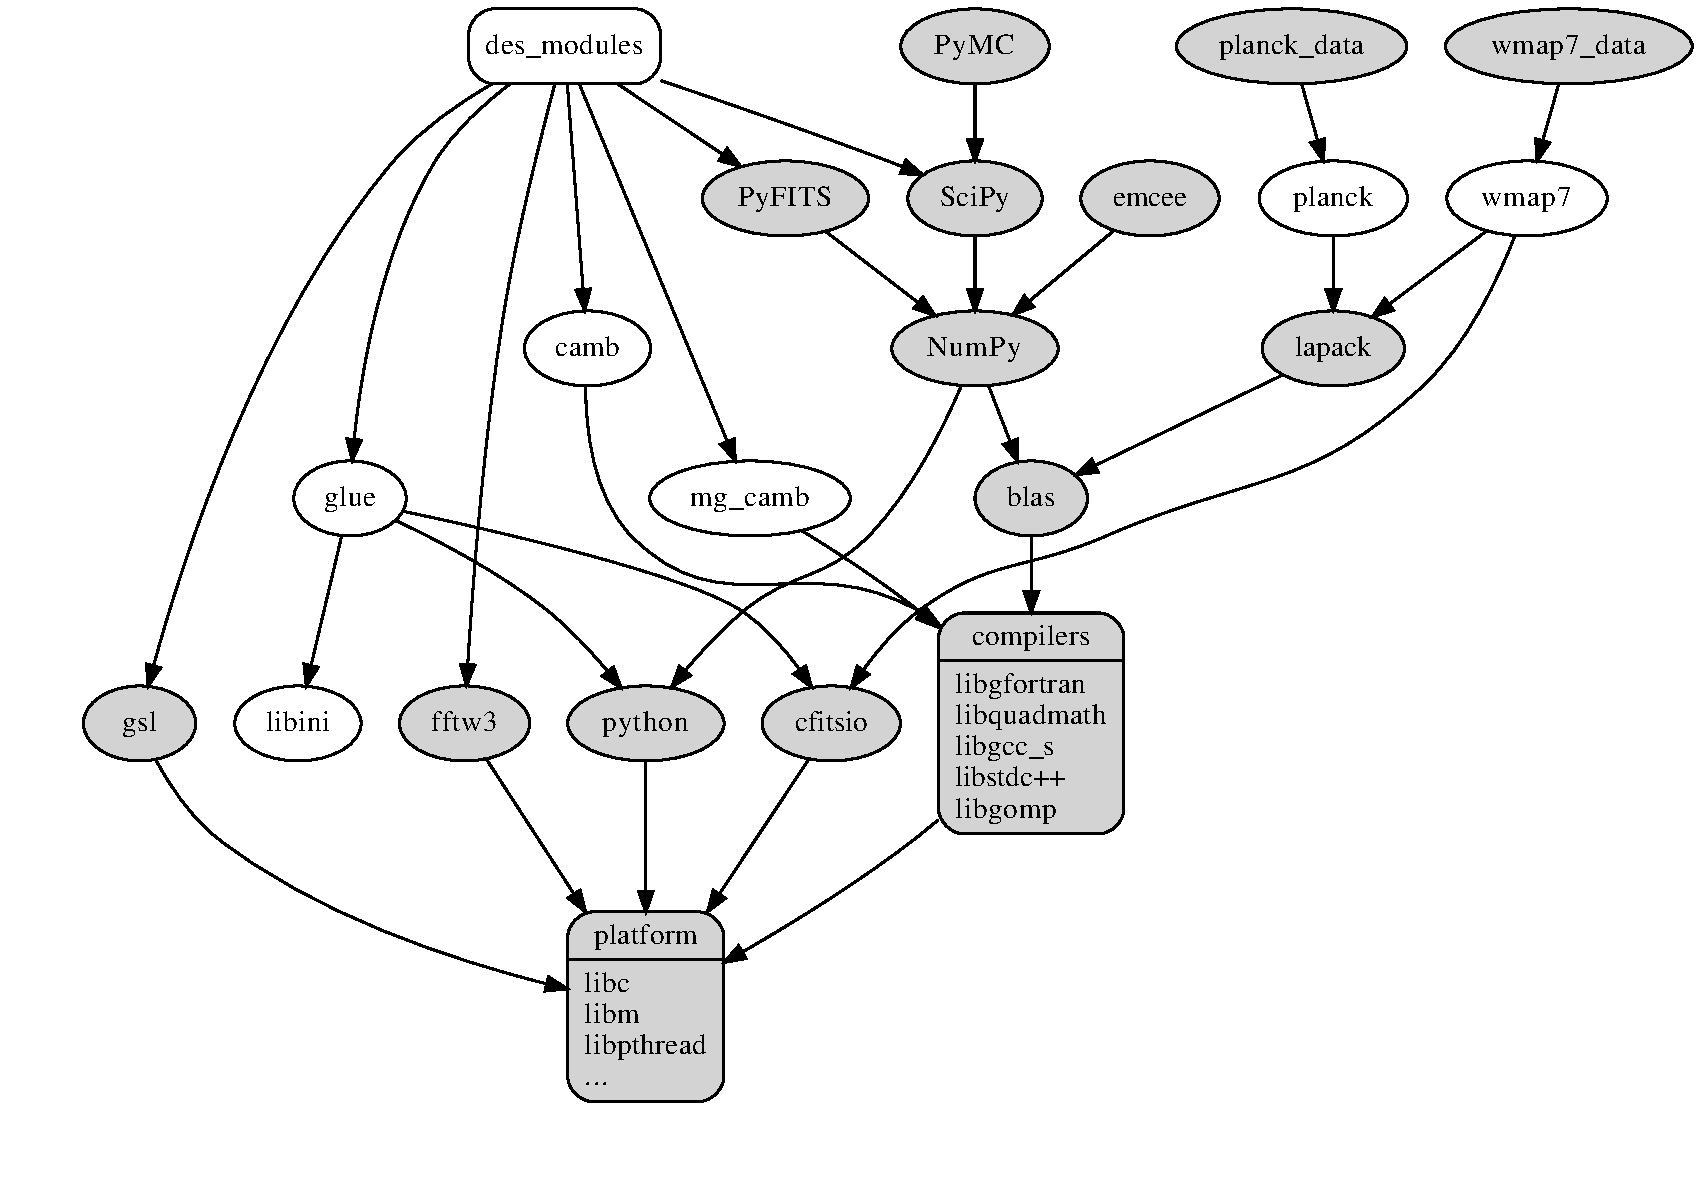
\includegraphics[width=\textwidth]{astro_packages}
  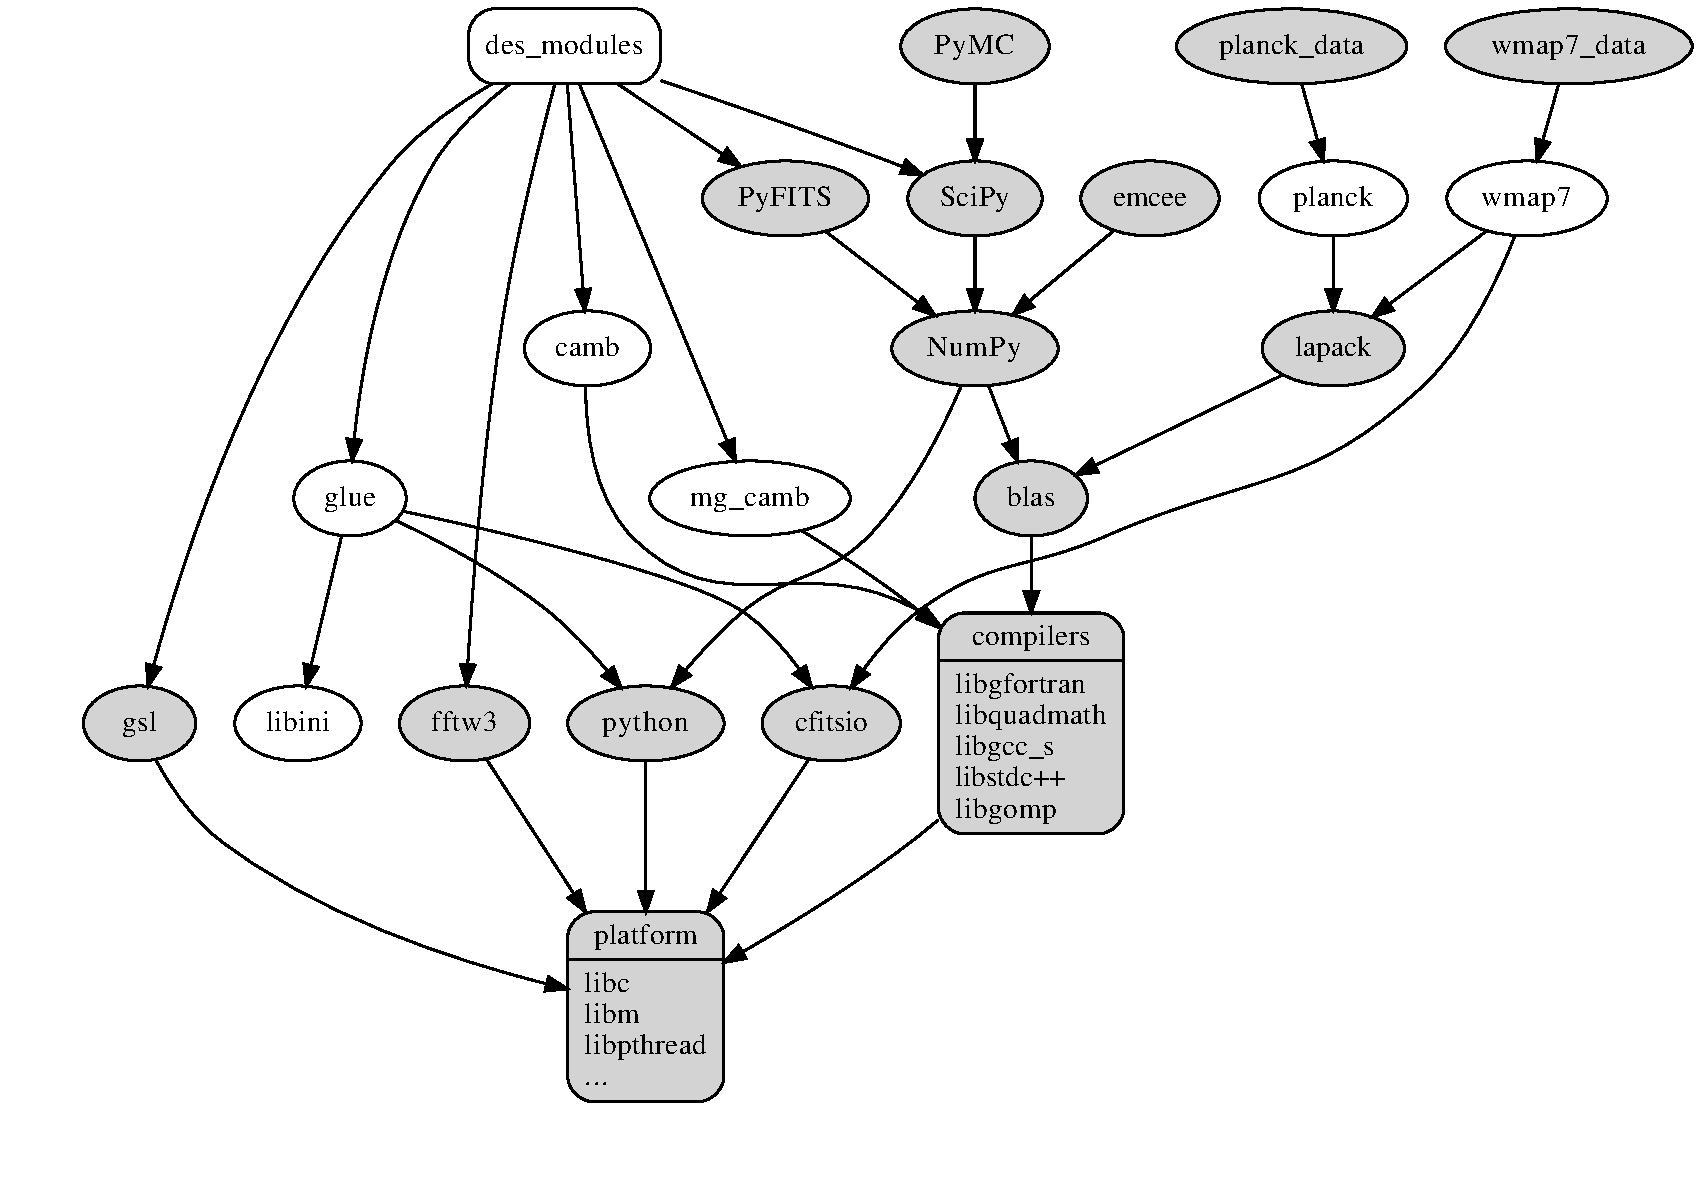
\includegraphics[width=\textwidth]{astro_packages}
}
\begin{fixme}
  These dependencies are not yet complete.
\end{fixme}
  \caption{Software packages currently part of the DES parameter
  estimation system. Rounded rectangles enclose groups of related
  code. Ellipses denote software products that are not grouped.}
  \label{fig:astropackages}
\end{figure}
\ifthenelse{\boolean{screen}}{\clearpage}{}


\subsection{Current build system}

For C and Fortran code, the \texttt{des-pipe} build system is based on
\name{make}, and consists of a set of Makefiles. For the Python code,
there is no build system; the user must have the software repository
available, and the Python environment correctly established to find the
Python modules of interest.

Building of each C or Fortran library is controlled independently, by the
individual Makefile for that module. Each Makefile can add or replace
compiler command-line switches and linker switches. This includes control over
the optimization level used by the C or Fortran compiler, what compiler
extensions are used (\eg, OpenMP), and what preprocessor variable
declarations are introduced (to control conditional compilation of
code).

There is no specific command to build all available modules. To build
each module, the user must execute the Makefile in each directory he is
interested in building. The user must have sufficient facility with
Makefile to be able to identify the targets of interest in each
Makefile.

Some Makefiles set compiler switches to values that can result in code that
is not compatible with code from other modules, \eg
\texttt{shear/becker/Makefile} sets the switch \texttt{-fshort-enums},
which produces code that in not binary-compatible with code generated
without that switch.
\subsection{Current development techniques}
\subsection{How programs are executed in the current system}


\chapter{Details}

We propose the establishment of several source code repositories for
DES-developed analysis source code, with one repository for each
identified group of related codes. Use of a source code version
control system will allow DES scientists to share code more easily,
and helps assure reproducible results, because all ``production''
versions of DES analysis modules will come from a known, and uniquely
identifiable, version of the DES source code.

\begin{fixme}
  For each section below, we should have the following issues covered:

  \begin{enumerate}
  \item Discussion
    \begin{itemize}
    \item Requirements
    \item Use cases
    \item Constraints
    \end{itemize}
  \item Possible directions
    \begin{itemize}
    \item Tools we use
    \item How it is now
    \item Where can it go?
    \end{itemize}
  \item Decisions
    \begin{itemize}
    \item What way should it go?
    \item What do users need to do as a result? How does existing code and practices need to change?
    \item What constraints/rules does it impose?
    \end{itemize}
  \end{enumerate}
\end{fixme}

\section{Framework}

We call the proposed framework \cosmosis. This is a framework
specifically for the creation of configurable Markov Chain Monte Carlo
parameter estimation programs. Each program consists of several
different types of components. These include:
\begin{itemize}
\item one \emph{sampler}, which is responsible for generating tuples
  in the parameter space according to some some sampling algorithm
  (possibly producing several tuples in parallel), and which invokes a
  \emph{likelihood function},
\item a \emph{likelihood function}, which is invoked by the sampler,
  to calculate the likelihood of the given parameter tuple; the
  likelihood function is composed from one or more \emph{physics
    modules},
\item a sequence of one or more \emph{physics modules} (see below).
\end{itemize}

The \emph{physics modules} are provided (though a standard interface)
the tuple of parameter values. Each physics module can read the values
of existing parameters, and calculate the values of new parameters
that it can then add to the tuple. The physics modules are run in a
sequence determined by a configuration file, supplied by the user, so
that later physics modules can access the values of parameters
calculated by earlier physics modules. Each physics module also can
(but need not) contribute to the calculation of the likelihood of the
parameter vector. Figure~\ref{fig:despes} shows the organization of a
\cosmosis program.

\ifthenelse{\boolean{screen}}{\clearpage}{}
\begin{figure}[htb]
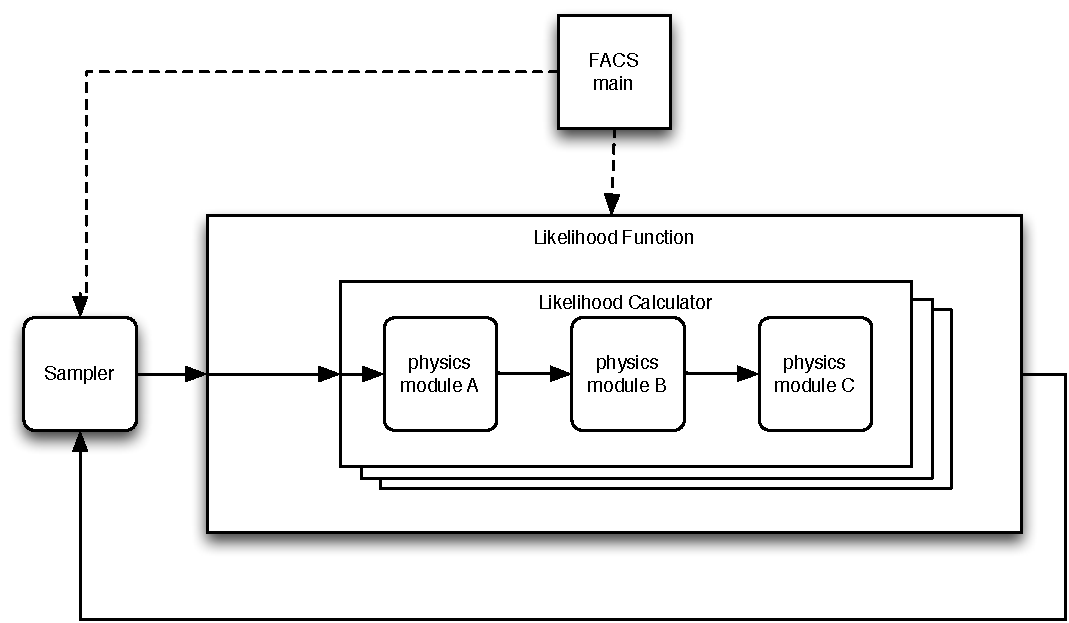
\includegraphics[width=\textwidth]{despes}
\caption{The organization of a \cosmosis program. Solid arrows
  show the flow of parameter data. Dotted arrows show the flow of
  configuration data. Modules may also read ancillary data files, as
  directed by their configuration. The multiple likelihood calculator
  boxes indicate the possible parallel processing of multiple
  parameter vectors produced by the sampler.}
\label{fig:despes}
\end{figure}
\ifthenelse{\boolean{screen}}{\clearpage}{}

% \subsection{Discussion}
% blah.
% \subsubsection{Requirements}
% blah.
% \subsubsection{Use cases}
% blah.
% \subsubsection{Constraints}
% blah.

% \subsection{Possible directions}
% blah.
% \subsubsection{Tools we use}
% blah.
% \subsubsection{Existing situation}
% blah.
% \subsubsection{Options}
% blah.

% \subsubsection{Decisions}
% blah.
% \subsubsection{Suggested solution}
% blah.
% \subsubsection{Changes to existing code and practice}
% blah.
% \subsubsection{Resulting rules and conventions}
% blah.

\section{Physics modules}

Physics modules perform calculations of two types. They accept as
input a collection of model parameters, and can augment the collection
with new parameters. They can not change the value of any existing
parameter. They can also calculate, and record, a likelihood value,
which will be combined with any other likelihoods calculated by other
modules in the program.

Physics modules are provided to the system by run-time configuration,
either through dynamically loaded libraries (for compiled languages)
or as Python modules.

Each physics module, at the time it is initialized, may be any data
files it needs to do its work. Typically, the names of the files to be
read will be supplied to the initialization code through the
framework's configuration mechanism.
% blah.
% \subsection{Discussion}
% blah.
% \subsubsection{Requirements}
% blah.
% \subsubsection{Use cases}
% blah.
% \subsubsection{Constraints}
% blah.

% \subsection{Possible directions}
% blah.
% \subsubsection{Tools we use}
% blah.
% \subsubsection{Existing situation}
% blah.
% \subsubsection{Options}
% blah.

% \subsubsection{Decisions}
% blah.
% \subsubsection{Suggested solution}
% blah.
% \subsubsection{Changes to existing code and practice}
% blah.
% \subsubsection{Resulting rules and conventions}
% blah.


\subsection{Samplers}


\subsection{Parameter calculators}

\subsection{Likelihood calculators}

\section{Configuration}

% \subsection{Discussion}
% blah.
% \subsubsection{Requirements}
% blah.
% \subsubsection{Use cases}
% blah.
% \subsubsection{Constraints}
% blah.

% \subsection{Possible directions}
% blah.
% \subsubsection{Tools we use}
% blah.
% \subsubsection{Existing situation}
% blah.
% \subsubsection{Options}
% blah.

% \subsubsection{Decisions}
% blah.
% \subsubsection{Suggested solution}
% blah.
% \subsubsection{Changes to existing code and practice}
% blah.
% \subsubsection{Resulting rules and conventions}
% blah.


\subsection{Whole program configuration}


\subsection{Module configuration}


\section{Packaging}


% \subsection{Discussion}
% blah.
% \subsubsection{Requirements}
% blah.
% \subsubsection{Use cases}
% blah.
% \subsubsection{Constraints}
% blah.

% \subsection{Possible directions}
% blah.
% \subsubsection{Tools we use}
% blah.
% \subsubsection{Existing situation}
% blah.
% \subsubsection{Options}
% blah.

% \subsubsection{Decisions}
% blah.
% \subsubsection{Suggested solution}
% blah.
% \subsubsection{Changes to existing code and practice}
% blah.
% \subsubsection{Resulting rules and conventions}
% blah.

\section{Provenance and storage}


% \subsection{Discussion}
% blah.
% \subsubsection{Requirements}
% blah.
% \subsubsection{Use cases}
% blah.
% \subsubsection{Constraints}
% blah.

% \subsection{Possible directions}
% blah.
% \subsubsection{Tools we use}
% blah.
% \subsubsection{Existing situation}
% blah.
% \subsubsection{Options}
% blah.

% \subsubsection{Decisions}
% blah.
% \subsubsection{Suggested solution}
% blah.
% \subsubsection{Changes to existing code and practice}
% blah.
% \subsubsection{Resulting rules and conventions}
% blah.


\section{Development environment and strategy}


% \subsection{Discussion}
% blah.
% \subsubsection{Requirements}
% blah.
% \subsubsection{Use cases}
% blah.
% \subsubsection{Constraints}
% blah.

% \subsection{Possible directions}
% blah.
% \subsubsection{Tools we use}
% blah.
% \subsubsection{Existing situation}
% blah.
% \subsubsection{Options}
% blah.

% \subsubsection{Decisions}
% blah.
% \subsubsection{Suggested solution}
% blah.
% \subsubsection{Changes to existing code and practice}
% blah.
% \subsubsection{Resulting rules and conventions}
% blah.

\chapter{Moving forward}

Priority, plans.

\chapter{Relationship to other work}

\begin{itemize}
\item Salman's project?
\item LSST DESC?
\end{itemize}

\appendix

\begin{thebibliography}{99}

\bibitem{des} The DES home page is \url{http://www.darkenergysurvey.org}.

\bibitem{numpy} \name{NumPy} is a Python library for scientific computing, available from \url{http://numpy.scipy.org}.

\bibitem{mercurial} \name{Mercurial} is a freely-available distributed
  version control system, available from
  \url{http://mercurial.selenic.com}.

\bibitem{bitbucket} \name{BitBucket} is an online service that
  provides hosting of Mercurial and Git repositories. It can be found
  at \url{https://bitbucket.org}.

\end{thebibliography}

\end{document}

%%% Local Variables:
%%% mode: latex
%%% TeX-master: t
%%% End:
